\chapter{基准折现率的确定}
基准折现率(基准收益率)是衡量项目可行性和方案比选的主要依据。它反映投资者对项目占用资金时间价值的判断,是投资者从事投资活动可接受的下临界值。其高低直接影响着经济评价决策指标的计算结果。如从$NPV(i)$的特性看,$i$定的越大,$NPV$越小,表明对项目要求越严,审查越严。

一个例子,你去玩一个游戏,赢了这个游戏给你100块钱,输了就什么都没有,输赢的概率都是50\%。此时给你两种选择:要么玩;要么你不参加游戏,直接给你50块钱。你的选择是?

那么,如果你去玩一个游戏,赢了这个游戏给你200块钱,输了就什么都没有,输赢的概率都是50\%。还是同样的两种选择:要么玩;要么你不参加游戏,直接给你50块钱。你的选择又是什么呢?

因此,我们确定基准折现率时,需考虑的因素如下:
机会成本、风险、资本成本、通胀。

\section{风险与收益}
\subsection{风险的概念}
风险是指投资者未来收益的不确定性。
\subsection{风险投资原则}
\begin{itemize}
    \item 同风险、同收益;
    \item 高风险,高收益;
    \item 低风险,低收益。
\end{itemize}

\subsection{股票、债券的报酬率}
\subsubsection{股票的报酬率}
$$\mbox{报酬率}=\mbox{股利收益率}+\mbox{资本利得收益率}=\frac{\mbox{期末支付的股利}+\mbox{当期市场价值的变动}}{\mbox{期初市场价值}}$$

\subsubsection{债券的报酬率}
通过长期的观察发现,债券的报酬率远低于股票的报酬率,国库券的报酬率很低。如买政府的国库券,几乎没有任何违约风险,此时的收益率可看成无风险报酬率。

\subsubsection{风险溢酬}
风险非常大的股票的报酬率和国库券的报酬率差额是超额报酬率。可以被解释为承担风险的报酬,称为\textbf{风险溢酬}。风险性资产会赚取风险溢酬,即承担风险就会有回报。而且通过对股票、债券等计算其\textbf{方差和标准差},发现报酬率越高,其标准差就越大,也就是在某一给定的年度,股票价值出现特别大的变动的机会就很大,说明收益率越高,风险越大。
$$\mbox{风险溢酬}=\mbox{期望报酬率}-\mbox{无风险报酬率}$$

\subsection{投资组合的报酬率及风险}

\begin{figure}[H]
    \centering
    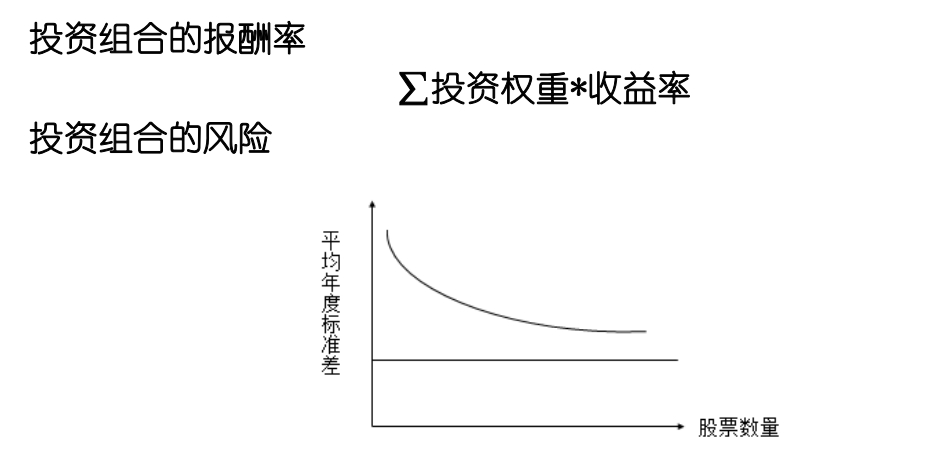
\includegraphics[width=0.9\textwidth]{image/投资组合的报酬率及风险.png}
    \caption{投资组合的报酬率及风险}
    \label{fig:10}
\end{figure}

\subsection{系统风险和非系统风险}
\textbf{系统风险(市场风险)}:对整个市场有影响,比如总体经济状况的不确定性,利率、经济衰退、战争等,属不可分散风险。

\textbf{非系统风险(特有风险或者具体资产风险)}:影响某个单项资产或一小组资产,是个别公司或者资产特有的,属可分散风险。
$$\mbox{整体风险}=\mbox{系统风险}+\mbox{非系统风险}$$

通过分散化化解非系统风险几乎没有任何成本,因此承担这种风险没有回报。
承担风险时所得到的回报的大小,仅取决于系统风险。也即一项资产的期望报酬率取决于系统风险。

通常用$\beta$衡量不同投资的系统风险水平。平均资产的$\beta$为1。

\begin{figure}[H]
    \centering
    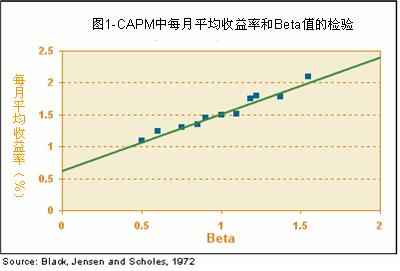
\includegraphics[width=0.8\textwidth]{image/CAPM中每月平均收益率和Beta值的检验.jpg}
    \caption{CAPM中每月平均收益率和Beta值的检验}
    \label{fig:11}
\end{figure}
$$\mbox{期望报酬率}=\mbox{无风险报酬率}+\mbox{市场风险溢酬}$$
$$R_E=R_f+[E(R_M)-R_f]*B_i$$

$R_f$:无风险报酬率;

$[E(R_M)-R_f]$:市场平均风险溢酬;

$B_i$:一项特定资产相对于平均资产而言,所面临的系统风险的大小。

\section{资本成本的确定}
\subsection{企业筹资的类别}
\textbf{权益资金(Equity)}是由企业所有者投入的资金,企业可长期使用,无需偿还。

\textbf{债务资金(Debt)}是由企业债权人投入的资金,企业需按约使用,按期偿还。

资本成本(cost of capital)是指投资者投资于企业的必要预期收益率。因此,资本成本与投资者投资于企业所承担的风险有关。

权益投资者承担相对较高的风险,因此权益资本成本较大。权益投资者承担的风险用贝塔系数来衡量。

债务投资者(债权人)承担相对较低的风险,因此债务成本较低。

\subsection{债务资本成本的计算}
\subsubsection{债券定价公式}
$$P=\sum_{t=1}^{n} \frac{I}{(1+r_D)^t}+\frac{F}{(1+r_D)^n}$$

$I$:各期的利息,等于票面值乘以票面利率。

$F$:债券面值。

$n$:债券到期期限。

$r_D$:债券的到期收益率,或债券资本成本。\\
\textbf{例题:}A公司发行的债券,面值为1000元,票面利率10\%,期限为10年。目前该债券还有8年到期,当前的市场价格为1050元。计算该债券的到期收益率或资本成本。\\
\textbf{答案:}
$$1050=\sum_{t=1}^{8}\frac{100}{(1+r_D)^t}+\frac{1000}{(1+r_D)^8}$$
$$r_D=9\%$$

\subsection{权益资本成本的计算}
利用资本资产定价模型(CAPM)
$$r_E=r_F+\beta \cdot (r_M-r_F)$$
式中:\\
$r_E$:权益必要收益率或权益资本成本;\\
$r_F$:无风险收益率;\\
$r_M$:市场平均收益率;\\
$\beta$:企业权益的风险系数。\\
\textbf{例题:}A公司的$\beta$系数为1.15,无风险收益率为6\%,市场平均收益率为14\%,计算A公司的权益资本成本。\\
\textbf{答案:}$r_E=6\%+1.15(14\%-6\%)=15.2\%$

\subsection{加权平均资本成本(WACC)}
个别资本成本为税后成本;个别资本的权重为市场价值权重。
$$WACC=\frac{D}{D+E} \times r_D(1-T)+\frac{E}{D+E}  \times r_E$$
式中:\\
$WACC$:加权平均资本成本;\\
$D$:债务的市场价值;\\
$E$:权益的市场价值;\\
$D+E$:企业的市场总价值。\\
\textbf{例题:}A公司现有债务4000万元,债务成本为9\%;权益价值6000万元,权益成本为15.2\%;该公司所得税税率为25\%,计算公司的WACC。\\
\textbf{答案:}$WACC=40\% \times 9\% \times (1-25\%) +60\% \times 15.2\%=11.82\%$

\section{投资风险补偿}
要估计一个适当的风险贴水率,也被称为风险补偿系数 (Risk Adjusted Discount Rate)
$$MARR=k+h$$

$K=Max$(借贷资金成本、加权平均资本成本、机会成本);

$h$:投资风险补偿系数。

\begin{table}[H]
\centering
\begin{tabular}{|l|l|}
\hline
\textbf{风险等级}       & \textbf{h(\%)}                \\ \hline
高度风险(新技术、新产品)      & 20\textasciitilde100        \\ \hline
较高风险(生产活动范围外新项目、新工艺) & 10\textasciitilde20         \\ \hline
一般风险(生产活动范围内市场信息不确切) & 5\textasciitilde10          \\ \hline
较小风险(已知市场现有生产外延)   & 1\textasciitilde5           \\ \hline
极小风险(稳定环境下降低生产费用)   & 0\textasciitilde1           \\ \hline
\end{tabular}
\caption{风险等级与风险百分比}
\end{table}

\section{通货膨胀}
若项目的收入和支出是各年的即时价格计算的必须考虑通货膨胀率;若按不变价格计算的,此项可不考虑。

\section{行业财务基准收益率的主要测定方法(了解即可)}
\subsection{资本资产定价模型}
不同行业的风险不同,风险溢价不同。通过测定行业投资收益变动与市场总投资收益变动的关系,分析行业投资风险的大小。在参数与方法中,行业财务基准收益率(权益资本)的测算采用了资本资产定价模型的思路与方法,并依据我国实际情况变通使用。

无风险收益率一般采用政府发行的相应期限的国债利率,2004年是2.5\%。市场平均风险投资收益率2004年是8\%。

\subsection{WACC(加权平均资本成本)}
通过测定WACC ,可以得出行业内全部投资的最低可用折现率,为确定融资前税前行业财务基准收益率提供参考价下限。在综合考虑各行业收益率并进行协调后,确定全行业基准投资收益率取值。

\subsection{典型项目模拟法}
通过选取行业内一定数量有代表性的已进入正常生产运营状态的建设项目,进行调查,搜集其折现率。当然,项目必须有代表性,典型。在一定典型的基础上,测定行业的。

\subsection{德尔菲专家调查法}
充分利用专家熟悉行业特点、行业发展变化规律、项目收益水平和具有丰富经验的优势,由一定数量的专家对项目收益率取值进行判断,经过几轮,逐步集中。形成结论性取值。

在调查过程中,如果在基本没有人为因素干扰的情况下能形成收敛性的结论,则这一结论能对基准收益率的取值提供重要参考。2006年时组织了全国500多位各行业专家进行调查。

\subsection{总结}
在测算中,无论哪种方法,都要在测算分析的基础上进行必要的调整,最终的取值是综合权衡的结果,而不是简单的计算。

国家行政部门统一测定、发布的行业基准财务收益率对于政府投资项目是规定性的,必须采用的,对于社会其他各类项目,是参考性的。项目评价人员可以根据具体情况选用,也可以自主测定。由投资者自己决定。

如石油行业的陆上气田开采项目,融资前财务基准收益率,专家调查结果是13\%,行业测算结果是12\%,协调结果是12\%。

\begin{figure}[H]
    \centering
    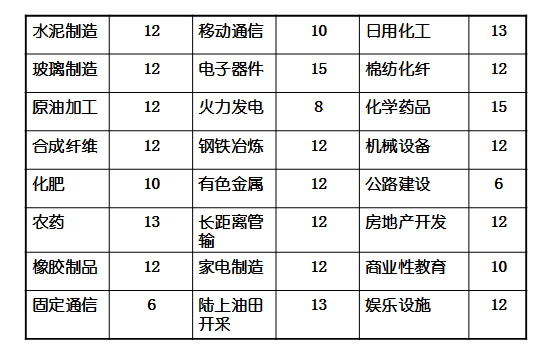
\includegraphics[width=0.9\textwidth]{image/我国行业基准折现率.png}
    \caption{我国行业基准折现率}
    \label{fig:12}
\end{figure}
